\chapter{Interferenza}%Interferenza
\section{Fenomeni di interferenza}%Fenomeni di interferenza
Quando la differenza di fase tra due onde in un qualsiasi punto è costante nel tempo le \b{sorgenti} delle due onde si dicono \b{coerenti}. Quando invece questa circostanza non si verifica, le \b{sorgenti} sono dette \b{incoerenti}.

Il termine \b{interferenza} è riferito propriamente ai fenomeni di sovrapposizione ottenuti con onde emesse da due o più sorgenti coerenti. \'E un fenomeno stazionario.

\subsection{Somma di due grandezze sinusoidalmente lungo lo stesso asse}
\subsubsection{Primo metodo - vettoriale}
Si supponga che due onde si propaghino lungo l'asse $x$, che vibrino lungo la stessa direzione e che il punto $P$ disti rispettivamente $x_1$ e $x_2$:
\begin{equation}\begin{split}
\xi_1=A_1\cos{\(kx_1-\omega t+\phi_1\)}=A_1\cos{\(\omega t-kx_1-\phi_1\)}=A_1\cos{\(\omega t+\alpha_1\)}\\
\xi_2=A_2\cos{\(kx_2-\omega t+\phi_2\)}=A_2\cos{\(\omega t-kx_2-\phi_2\)}=A_2\cos{\(\omega t+\alpha_2\)}
\end{split}\end{equation}
interferendo si ha:
\begin{equation}\begin{split}
\xi=\xi_1+\xi_2=A\cos{\(\omega t+\alpha\)}
\end{split}\end{equation}
dove il \b{modulo} è:
\begin{equation}\begin{split}
A=\sqrt{A_1^2+A_2^2+2A_1A_2\cos{\delta}}\\
\delta=\alpha_1-\alpha_2=\phi_2-\phi_1+k\(x_2-x_1\)
\end{split}\end{equation}
e la \b{fase} è:
\begin{equation}\begin{split}
\tan{\alpha}=\frac{A_1\sin{\alpha_1}+A_2\sin{\alpha_2}}{A_1\cos{\alpha_1}+A_2\cos{\alpha_2}}
\end{split}\end{equation}

L'\b{intensità misurata} nel punto $P$ è:
\begin{equation}\begin{split}
I=I_1+I_2+2\cos{\delta}\sqrt{I_1I_2}
\end{split}\end{equation}

Se le \b{ampiezze sono uguali} si ha:
\begin{equation}\begin{split}
A=\sqrt{2A_0^2\(1+\cos{\delta}\)}=2A_0\cos{\frac{\delta}{2}}
\end{split}\end{equation}
\begin{equation}\begin{split}
\alpha=\frac{\alpha_1+\alpha_2}{2}
\end{split}\end{equation}
e l'onda risultante è:
\begin{equation}\begin{split}
\xi=A\cos{\(\omega t+\alpha\)}=2A_0\cos{\[\frac{\phi_2-\phi_1}{2}+\frac{k\(x_2-x_1\)}{2}\]}\cos{\[\frac{\phi_2+\phi_1}{2}+\frac{k\(x_2+x_1\)}{2}-\omega t\]}
\end{split}\end{equation}
e l'intensità vale:
\begin{equation}\begin{split}
I=2I_0\(1+\cos{\delta}\)=4I_0\cos^2{\frac{\delta}{2}}
\end{split}\end{equation}
e quindi \b{l'ampiezza della somma dipende dalla differenza di fase}: il valore massimo si ha quando le onde sono in fase, il minimo quando sono in opposizione.

\subsubsection{Secondo metodo - simbolico}
Utilizza i numeri complessi. E si ha:
\begin{equation}\begin{split}
\xi_1=A_1e^{i\(\omega t+\alpha_1\)}=A_1\cos{\(\omega t+\alpha_1\)}+iA_1\sin{\(\omega t+\alpha_1\)}\\
\xi_2=A_2e^{i\(\omega t+\alpha_2\)}=A_2\cos{\(\omega t+\alpha_2\)}+iA_2\sin{\(\omega t+\alpha_2\)}
\end{split}\end{equation}
\begin{equation}\begin{split}
\xi=\\
\xi_1+\xi_2=\(A_1e^{i\alpha_1}+A_2E^{i\alpha_2}\)e^{i\omega t}=\\
\[A_1\cos{\alpha_1}+A_2\cos{\alpha_2}+i\(A_1\sin{\alpha_1}+A_2\sin{\alpha_2}\)\]e^{i\omega t}
\end{split}\end{equation}
\begin{equation}\begin{split}
\xi\xi^*=\\
\(A_1e^{i\alpha_1}+A_2e^{i\alpha_2}\)e^{i\omega t}\(A_1e^{-i\alpha_1}+A_2e^{-i\alpha_2}\)e^{-i\omega t}=\\
A_1^2+A_2^2+2A_1A_2\cos{\(\alpha_1-\alpha_2\)}
\end{split}\end{equation}
con $\xi^*$ il complesso coniugato.

\subsection{Somma di due oscillazioni armoniche sullo stesso asse}
\begin{center}
\begin{tabularx}{\textwidth}{l| c cc cc}
\toprule
		& Sfasamento 		& \multicolumn{2}{c}{Ampiezze diverse} 			& \multicolumn{2}{c}{Ampiezze uguali} \\
\midrule
max 		& $\delta=0,2\pi$ 	& $A=A_1+A_2$ 	& $I=I_1+I_2+2\sqrt{I_1I_2}$ 	& $A=2A_0$ 	& $I=4I_0$ \\
min 		& $\delta=\pi,3\pi$ 	& $A=|A_1-A_2|$ 	& $I=I_1+I_2-2\sqrt{I_1I_2}$ 	& $A=0$ 		& $I=0$ \\
\bottomrule
\end{tabularx}
\end{center}

\section{Interferenza prodotta da due sorgenti}%Interferenza prodotta da due sorgenti
Si hanno due sorgenti coerenti di onde armoniche sferiche con la stesa pulsazione $\omega$ che si propagano in un mezzo indefinito isotropo con velocità $v$, lunghezza d'onda $\lambda=\frac{v}{\nu}$ e numero d'onda $k=\frac{\omega}{v}$:
\begin{equation}\begin{split}
\xi_1=\frac{\xi_0}{r_1}\cos{\(kr_1-\omega t\)}\\
\xi_2=\frac{\xi_0}{r_2}\cos{\(kr_2-\omega t\)}
\end{split}\end{equation}

\subsection{Onde trasversali con la stessa direzione di vibrazione}
\begin{center}
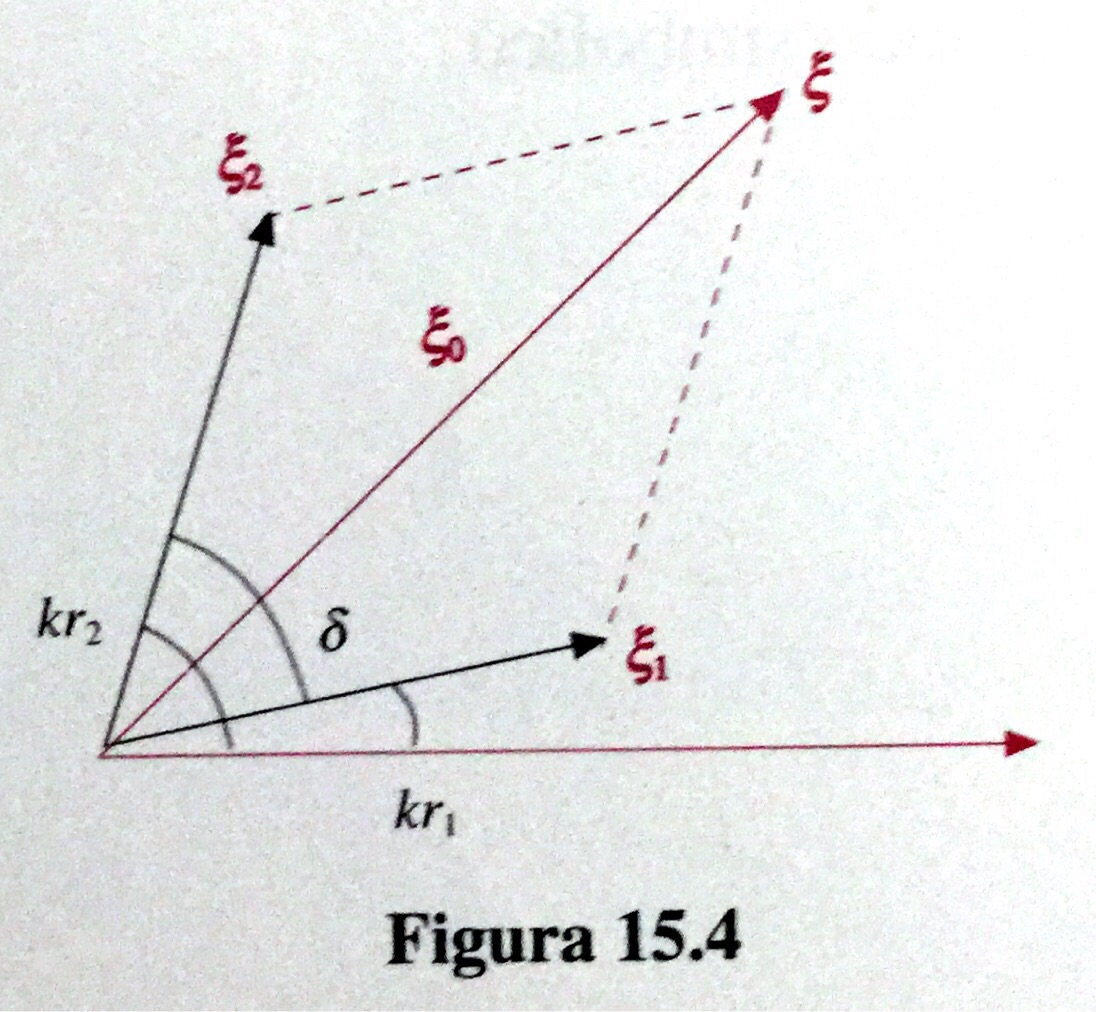
\includegraphics[width=2in]{immagini/InterfFoto.jpg}
\end{center}

Nel punto $Q$ (per essere trovato in modo finito si usano lenti convergenti) hanno la stessa direzione di vibrazione, così da poterle trattare nella somma come quantità scalari; considerando inoltre il \b{principio di Fermat} che dice che le lenti non introducono sfasamenti, si ha l'\b{ampiezza dell'onda risultante} nel punto $Q$:
\begin{equation}\begin{split}
\xi_0=\sqrt{\xi_{0,1}^2+\xi_{0,2}^2+2\xi_{0,1}\xi_{0,2}\cos{\delta}},
\end{split}\end{equation}
la \b{differenza di fase costante} è:
\begin{equation}\begin{split}
\delta=k\(r_2-r_1\)=\frac{2\pi}{\lambda}\(r_2-r_1\).
\end{split}\end{equation}
L'\b{intensità} è invece:
\begin{equation}\begin{split}
I=I_1+I_2+2\cos{\[\frac{2\pi}{\lambda}\(r_2-r_1\)\]}\sqrt{I_1I_2}.
\end{split}\end{equation}

Si dice che l'\b{interferenza} è \b{costruttiva} se:
\begin{equation}\begin{split}
\delta=2m\pi, \qquad \Delta r=r_2-r_1=m\lambda, \qquad m=0,\pm 1,\pm 2,\dots
\end{split}\end{equation}
mentre che l'\b{interferenza} è \b{distruttiva} se:
\begin{equation}\begin{split}
\delta=\(2m'+1\)\pi, \qquad \Delta r=r_2-r_1=\(2m'+1\)\frac{\lambda}{2}, \qquad m'=0,\pm 1,\pm 2,\dots
\end{split}\end{equation}

In un qualsiasi piano contenente le due sorgenti, la condizione $r_2-r_1=\const$ individua una coppia di iperboli aventi le due sorgenti come fuochi. Le superfici di massima intensità si dicono \b{superfici ventrali}, quelle di minima intensità \b{superfici nodali}.

\subsection{Punto $Q$ a distanza molto maggiore della distanza tra le sorgenti}
Si ha la distanza dal punto medio $r$ e la distanza tra le sorgenti $d$:
\begin{equation}\begin{split}
r_2-r_1=d\sin{\theta}, \qquad \delta=\frac{2\pi}{\lambda}d\sin{\theta}.
\end{split}\end{equation}

L'\b{ampiezza} è
\begin{equation}\begin{split}
\xi_0=\sqrt{2\xi_{0,1}^2\(1+\cos{\delta}\)}=2\xi_{0,1}\cos{\frac{\delta}{2}}=2\xi_{0,1}\cos{\(\frac{\pi d\sin{\theta}}{\lambda}\)}
\end{split}\end{equation}
e l'\b{intensità} è:
\begin{equation}\begin{split}
I\(r,\theta\)=4I_1\cos^2{\frac{\delta}{2}}=4I_1\cos^2{\(\frac{\pi d\sin{\theta}}{\lambda}\)}, \qquad I_1=\frac{P}{4\pi r^2}
\end{split}\end{equation}

Si dice che l'\b{interferenza} è \b{costruttiva} se:
\begin{equation}\begin{split}
\sin{\theta}=m\frac{\lambda}{d}, \qquad m=0,\pm 1,\pm 2,\dots
\end{split}\end{equation}
mentre che l'\b{interferenza} è \b{distruttiva} se:
\begin{equation}\begin{split}
\sin{\theta}=\(2m'+1\)\frac{\lambda}{2d}, \qquad m=0,\pm 1,\pm 2,\dots
\end{split}\end{equation}

\section{Interferenza di due onde luminose}%Interferenza di due onde luminose
Sia le onde provenienti da due punti di una sorgente estesa che le onde provenienti da due sorgenti diverse risultano essere incoerenti e non danno luogo a fenomeni di interferenza.

\subsection{Esperimento di Young}
Una fascio di luce ordinaria monocromatica incide su uno schermo in cui è praticata una fenditura $S_0$ lunga e sottile, che funge da sorgente primaria dell'esperimento. Le onde uscenti da questa fenditura arrivano su un secondo schermo in cui sono praticate due fenditure sottili $S_1$ e $S_2$, parallele alla precedente ed equidistanti dall'asse del dispositivo; le due fenditure agiscono come coppia di sorgenti coerenti.

La luce emessa da $S_1$ e $S_2$ produce su uno schermo $C$, posto a distanza $L$ dalle sorgenti, grande rispetto alla loro separazione, una figura visibile, detta \b{figura di interferenza}, che consiste in una serie di strisce chiare e scure, parallele alle fenditure chiamate \b{frange d'interferenza}. Le frange chiare corrispondono ai massimi, quelle scure ai minimi di intensità.

I fattori che rendono le frange poche o di poca intensità sono:
\begin{itemize}
\item obliquità: nell'intensità $I_1$ compare il quadrato del \b{fattore di inclinazione}:
\begin{equation}\begin{split}
f^2\(\theta\)=\(\frac{1+\cos{\theta}}{2}\)^2;
\end{split}\end{equation}
\item diffrazione;
\item larghezza delle fenditure;
\item coerenza.
\end{itemize}

Si può supporre che $\sin{\theta}\simeq\tan{\theta}\simeq\theta=\frac{x}{L}$ e quindi:
\begin{equation}\begin{split}
I\(x\)=4I_1\cos^2{\(\frac{\pi dnx}{\lambda_0L}\)}
\end{split}\end{equation}
e quindi si ha il \b{massimo} per
\begin{equation}\begin{split}
\theta=m\frac{\lambda_0}{nd}, \qquad x=m\frac{\lambda_0L}{nd}
\end{split}\end{equation}
e il \b{minimo} per
\begin{equation}\begin{split}
\theta=\(2m'+1\)\frac{\lambda_0}{2nd}, \qquad x=\(2m'+1\)\frac{\lambda_0L}{2nd}
\end{split}\end{equation}
dove $\lambda_0$ è la lunghezza d'onda nel vuoto e $\lambda=\frac{\lambda_0}{n}$ la lunghezza d'onda nel mezzo.

Essendo $d\gg\lambda$, la successione di massimi e minimi è molto frequente. Il passo dei massimi è $\Delta x=\frac{\lambda_0L}{nd}$. \'E essenziale anche che $d\ll L$ per osservare le frange d'interferenza. Affinché si formi la figura d'interferenza occorre che i campi elettrici $\E_1$ e $\E_2$ delle due onde siano polarizzati secondo la medesima direzione.

Le onde emesse dalle sorgenti $S_1$ e $S_2$ non sono onde armoniche, per questo motivo per poter osservare l'interferenza si sovrappongono quasi totalmente i due pacchetti d'onde provenienti da $S_1$ e $S_2$, originati dallo stesso pacchetto proveniente da $S_0$: solo così la differenza di fase e il piano di polarizzazione dei due campi rimangono costanti durante tutto il tempo in cui si sovrappongono.

Questo è valido finché la differenza di cammino che i due pacchetti devono percorrere per raggiungere lo stesso punto dello schermo è molto minore della loro lunghezza $\Delta x$ che viene chiamata \b{lunghezza di coerenza} che vale \SI{3}{\metre}. Viene definito anche il \b{tempo di coerenza} $\Delta t$ che vale \SI{e-8}{\second}.

\subsection{Cammino ottico}
La differenza di fase dovuta a una differenza di cammino geometrico è $\delta=k_2r_2-k_1r_1$. Nel vuoto vale:
\begin{equation}\begin{split}
\delta=k_0\(n_2r_2-n_1r_1\)=\frac{2\pi}{\lambda_0}\(n_2r_2-n_1r_1\)
\end{split}\end{equation}
definendo $n_ir_i$ il \b{cammino ottico}.

\subsection{Lenti e specchi}
\subsubsection{Lenti convergenti}
Un fascio di raggi paralleli all'asse della lente viene fatto convergere da questa in un punto $F$ detto \b{fuoco}, distante $f$ (chiamata \b{distanza focale}) dalla lente, mentre un fascio di raggio formanti un angolo $\theta$ piccolo con l'asse della lente converge in un punto $Q$ del piano focale, che è il piano ortogonale all'asse passante per il fuoco.

Il raggio passante per il centro della lente non viene deviato. La lente non introduce sfasamenti tra i vari raggi.

\subsubsection{Specchi piani}
Dato un punto $S$ che invia raggi allo specchio, i raggi riflessi sembrano provenire da un punto $S'$ (chiamato \b{immagine virtuale}) che è il simmetrico di $S$ rispetto al piano dello specchio.

\section{Applicazioni del metodo di Young}%Applicazioni del metodo di Young

\subsection{Specchi di Fresnel}
La luce emessa da una sorgente puntiforme incide su due specchi piani, che formano tra loro un angolo molto piccolo. \'E come se la luce provenisse dalle due immagini virtuali date dagli specchi, le quali fungono da sorgenti coerenti di onde di uguale intensità.

\subsection{Specchio di Lloyd}
La luce monocromatica proveniente da una fenditura illuminata, posta a distanza $\frac{d}{2}$ sopra il piano di una lastra di vetro, raggiunge lo schermo sia direttamente che per riflessione sulla lastra con grande angolo di incidenza. Le sorgenti coerenti sono la sorgente e la sua immagine virtuale. Le posizioni di massimi e minimi sono invertite.

\subsection{Biprisma di Fresnel}
Due lastre di vetro a sezione triangolare (prismi) sono accostante lungo le basi. La sorgente invia luce verso lo schermo e, a causa della rifrazione sui prismi, la luce sempre provenire da due punti che sono le sorgenti virtuali del sistema. Le frange osservate sono simili a quelle ottenute dagli specchi di Fresnel.

\subsection{Interferometro per la misura degli indici di rifrazione dei gas}
\`E formato da una lente $L_1$ che trasforma il fascio di luce divergente da una sottile fenditura $S_0$ illuminata, posta nel fuoco della lente, in un fascio parallelo, due tubi $T_1$ e $T_2$ paralleli uguali, di lunghezza $h$, con finestre trasparenti, due fenditure $S_1$ e $S_2$ parallele alla prima e infine una lente $L_2$ che permette la formazione su uno schermo posto nel suo piano focale della figura di interferenza prodotta dalle due fenditure.

Supponendo che inizialmente nei tubi ci sia il vuoto, nel centro dello schermo si forma la frangia chiara di ordine 0 e la frangia di ordine $m$ si forma nel punto tale che $r_1-r_2=m\lambda_0$; la differenza di fase deriva unicamente dalla differenza di cammino geometrico dopo le fenditure.

Se $T_1$ è riempito con un gas a pressione tale che l'indice di rifrazione sia $n$, i cammini ottici nei tubi non sono uguali e esiste una \b{differenza di fase} $k_1h-k_0h=nk_0h-k_0h=k_0\(n-1\)h$. Tutto il sistema si è spostato rigidamente verso l'alto di:
\begin{equation}\begin{split}
N=m'-m=\frac{\(n-1\)h}{\lambda_0}
\end{split}\end{equation}

\subsection{Interferometro di Fizeau}
Dopo le due fenditure di un dispositivo di Young è posta una lente convergente e uno schermo, coincidente col piano focale della lente.

Venne usato per misurare la separazione angolare tra due fasci di luce provenienti da sorgenti molto lontane. Ciascuna sorgente lontana produce una figura di interferenza sullo schermo. \'E possibile che i massimi di una figura coincidano con i minimi dell'altra, dando uno schermo uniformemente illuminato se l'intensità delle sorgenti è la stessa o facendo apparire zone più chiare o meno chiare.

La condizione di scomparsa della figura di interferenza si verifica quando la differenza di cammino lungo la direzione inclinata è multipla, secondo un numero intero dispari, di $\frac{\lambda}{2}$ ovvero quando:
\begin{equation}\begin{split}
\theta=\frac{\lambda}{2d}\(2m+1\).
\end{split}\end{equation}

\subsubsection{Misura separazione angolare tra due stelle}
Si aumenta la distanza $d$ tra le due fenditure fino a raggiungere il valore $d_1$ tale che lo schermo sia uniformemente illuminato, per cui vale $\theta=\frac{\lambda}{2d_1}\(2m+1\)$. Si aumenta di nuovo $d$ fino al nuovo valore $d_2$ per il quale lo schermo è di nuovo uniformemente illuminato, cioè $\theta=\frac{\lambda}{2d_2}\[2\(m+1\)+1\]$. Combinando le equazioni si ha:
\begin{equation}\begin{split}
m=\frac{3d_1-d_2}{2\(d_2-d_1\)}, \qquad \theta=\frac{\lambda}{d_2-d_1}.
\end{split}\end{equation}

\section{Interferenza prodotta da $N$ sorgenti coerenti}%Interferenza prodotta da $N$ sorgenti coerenti
Si consideri $N$ sorgenti uguali di onde sferiche, coerenti, disposte lungo una retta ed equispaziate di una distanza $d$ e si supponga di osservare la loro interferenza ad una distanza molto grande rispetto alla dimensione lineare $\(N-1\)d$ del sistema.
\begin{center}
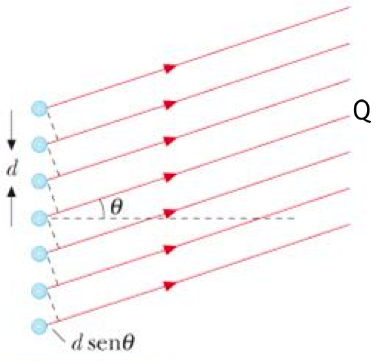
\includegraphics[width=2in]{immagini/interfN1.png}
\end{center}
Detto $\theta$ l'angolo formato tra la direzione di osservazione e la normale alla linea contenente le sorgenti, tra due onde emesse da due sorgenti consecutive esiste la differenza di fase:
\begin{equation}\begin{split}
\delta=\frac{2\pi}{\lambda}d\sin{\theta}=kd\sin{\theta}
\end{split}\end{equation}
\begin{center}
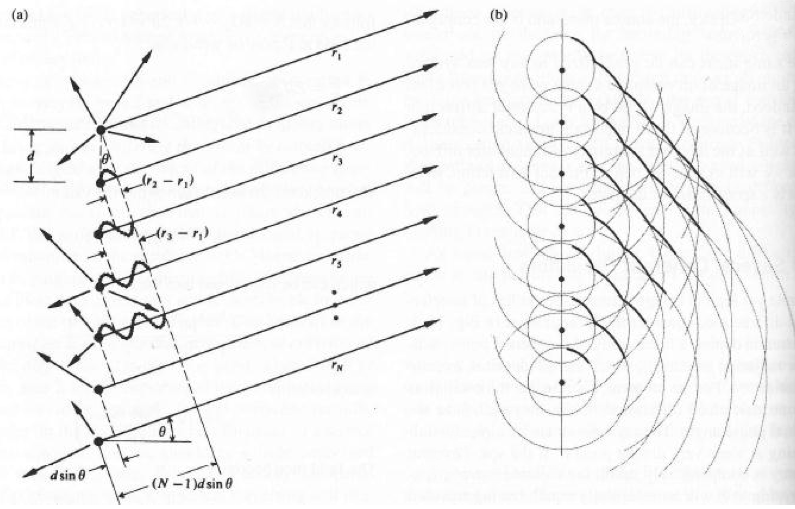
\includegraphics[width=5.5in]{immagini/interfN2.png}
\end{center}

In un punto $Q$ le ampiezze delle singole onde sferiche sono uguali; non sono invece uguali le fasi a causa delle differenze di cammino.
\begin{center}
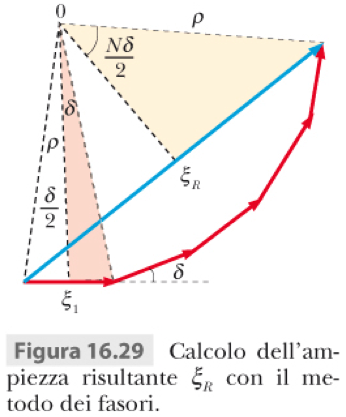
\includegraphics[width=2.5in]{immagini/interfampfas.png}
\end{center}

\subsubsection{Metodo vettoriale}
Le singole ampiezze $\xi_1$ si dispongono lungo una poligonale regolare di $N$ lati, che è circoscrivibile con una circonferenza di centro $O$ e raggio $\rho$; l'angolo al centro che sottende il singolo vettore è $\delta$, quello che sottende la poligonale è $N\delta$:
\begin{equation}\begin{split}
\xi_1=2\rho\sin{\frac{\delta}{2}}, \qquad \xi_R=2\rho\sin{\frac{N\delta}{2}}=\xi_1\frac{\sin{\frac{N\delta}{2}}}{\sin{\frac{\delta}{2}}}
\end{split}\end{equation}
con $\xi_R$ l'ampiezza risultante e l'intensità dell'onda risultante è:
\begin{equation}\begin{split}
I_R\(\theta\)=\\
I_1\(\frac{\sin{\frac{N\delta}{2}}}{\sin{\frac{\delta}{2}}}\)^2=\\
I_{ 1 }\[\frac { \sin { \(\frac { N\pi d\sin { \theta  }  }{ \lambda  } \) }  }{ \sin { \(\frac { \pi d\sin { \theta  }  }{ \lambda  } \) }  } \]^{ 2 }
\end{split}\end{equation}
dove $I_1$ è l'intensità che la singola sorgente produce nel punto $Q$.

\subsubsection{Metodo simbolico}
Si ha:
\begin{equation}\begin{split}
\widetilde E=\\
E_0\(r\)\sum_{n=1}^N{e^{i\(kr_n-\omega t\)}}=\\
E_0\(r\)e^{-i\omega t}e^{ikr_1}\[1+\sum_{n=2}^N{e^{ik\(r_{n}-r_1\)}}\]
\end{split}\end{equation}
e ponendo $\delta=k\(r_2-r_1\)$, $2\delta=k\(r_3-r_1\)$ e così via si ha:
\begin{equation}\begin{split}
E_0\(r\)e^{-i\omega t}e^{ikr_1}\[1+\sum_{n=1}^{N-1}{\(e^{i\delta}\)^n}\]
\end{split}\end{equation}
\begin{equation}\begin{split}
\frac{e^{iN\delta}-1}{e^{i\delta}-1}=\frac{e^{iN\frac{\delta}{2}}\(e^{iN\frac{\delta}{2}}-e^{-iN\frac{\delta}{2}}\)}{e^{i\frac{\delta}{2}}\(e^{i\frac{\delta}{2}}-e^{-i\frac{\delta}{2}}\)}=e^{i\(N-1\)\frac{\delta}{2}}\frac{\sin{N\frac{\delta}{2}}}{\sin{\frac{\delta}{2}}}
\end{split}\end{equation}
e quindi:
\begin{equation}\begin{split}
\widetilde E=E_0\(r\)e^{-i\omega t}e^{i\[kr_1+\(N-1\)\frac{\delta}{2}\]}\frac{\sin{N\frac{\delta}{2}}}{\sin{\frac{\delta}{2}}}
\end{split}\end{equation}

Poiché $R=\frac{1}{2}\(N-1\)d\sin{\theta}+r_1$ è la distanza dalla sorgente centrale $Q$, si ha il \b{campo risultante}:
\begin{equation}\begin{split}
\widetilde E=E_0\(r\)e^{i\(kR-\omega t\)}\frac{\sin{N\frac{\delta}{2}}}{\sin{\frac{\delta}{2}}}
\end{split}\end{equation}
e l'\b{intensità risultante}:
\begin{equation}\begin{split}
I=\\
I_0\(\frac{\sin{N\frac{\delta}{2}}}{\sin{\frac{\delta}{2}}}\)^2=\\
I_0\[\frac { \sin { \(Nk\frac { d }{ 2 } \sin { \theta  } \) }  }{ \sin { \(k\frac { d }{ 2 } \sin { \theta  } \) }  } \]^{ 2 }
\end{split}\end{equation}

\subsection{Massimi e minimi}
Ponendo $N=2$ si trova:
\begin{equation}\begin{split}
I_R\(\theta\)=4I_1\cos^2{\frac{\delta}{2}}.
\end{split}\end{equation}
L'\b{intensità varia con l'angolo di osservazione}.

Considerando $\theta=0, \pi, 2\pi, \dots$, direzione lungo la quale le onde sono tutte in fase: l'intensità è massima e vale $I_{\max}=N^2I_1$ in quanto $\lim_{x\to\infty}{\frac{\sin{Nx}}{\sin{x}}}=N$ e quindi $\xi_R=N\xi_1$.

L'\b{intensità presenta nell'intervallo $0\le\theta\le\frac{\pi}{2}$ un certo numero di massimi principali}:
\begin{equation}\begin{split}
\frac{\pi d\sin{\theta}}{\lambda}=m\pi \Longrightarrow d\sin{\theta}=m\lambda, \qquad \sin{\theta}=m\frac{\lambda}{d}
\end{split}\end{equation}
per quanto riguarda invece i \b{minimi}:
\begin{equation}\begin{split}
\frac{N\pi d\sin{\theta}}{\lambda}=m'\pi \Longrightarrow d\sin{\theta}=m'\frac{\lambda}{N}, \qquad \sin{\theta}=m'\frac{\lambda}{Nd}
\end{split}\end{equation}
escludendo i valori multipli pari di $N$.

\b{Tra due massimi principali ci sono $N-2$ massimi secondari} che si ottengono quando il numeratore di $I_R$ vale 1, cioè in corrispondenza a:
\begin{equation}\begin{split}
\sin{\theta}=\(2m''+1\)\frac{\lambda}{2Nd}
\end{split}\end{equation}
che porta ad un'intensità di:
\begin{equation}\begin{split}
I_m=\frac{I_{\max}}{N^2\[\sin{\frac{\(2m''+1\)\pi}{2N}}\]^2}.
\end{split}\end{equation}

Le principali \b{caratteristiche} sono:
\begin{itemize}
\item la posizione dei massimi principali, nei quali è concentrata la maggior parte della potenza emessa, è determinata dal rapporto $\frac{\lambda}{d}$ e non dipende dal numero delle sorgenti;
\item l'intensità dei massimi principali dipende dal numero delle sorgenti e cresce con questo secondo $I_{\max}=N^2I_1$;
\item l'ampiezza angolare dei massimi principali diminuisce all'aumentare di $N$. La \b{larghezza angolare di un massimo principale} viene definita come distanza tra i due minimi adiacenti al massimo:
\begin{equation}\begin{split}
\Delta\(\sin{\theta}\)=\frac{2\lambda}{Nd};
\end{split}\end{equation}
\item gli $N-1$ minimi e gli $N-2$ massimi secondari compresi tra due massimi principali sono equispaziati nella variabile $\sin{\theta}$: l'intervallo tra un minimo e un massimo secondario è $\frac{\lambda}{2}Nd$, l'intervallo tra due estremi consecutivi dello stesso tipo è $\frac{\lambda}{N}d$.
\end{itemize}

\section{Interferenza delle onde luminose su lamine sottili}%Interferenza delle onde luminose su lamine sottili
L'interferenza dovuta alla riflessione della luce sulle due superfici di una lamina sottile di una sostanza trasparente è il caso di interferenza più facile da osservare nella vita comune.

\subsubsection{Lamina sottile spessa $d$, formata da una sostanza trasparente con indice di rifrazione $n_2$ e immerso in un mezzo con indice di rifrazione $n_1$}
Si supponga di osservare a piccoli angoli rispetto la normale: una parte della luce incidente sulla lamina è riflessa dalla superficie superiore; l'onda trasmessa si propaga nella lamina ed è parzialmente riflessa dalla superficie inferiore; la parte riflessa riattraversa la lamina ed emerge nel primo mezzo con direzione parallela a quella del primo raggio riflesso.

Le due onde giungono all'occhio sfasate sia per la differenza di cammino ottico sia per lo sfasamento $\pi$ subito alla prima o alla seconda riflessione.

L'interferenza è prodotta da \b{due onde sfasate complessivamente} di:
\begin{equation}\begin{split}
\delta=\frac{4\pi n_2d}{\lambda_0}+\pi.
\end{split}\end{equation}

L'interferenza è \b{costruttiva} se:
\begin{equation}\begin{split}
\delta=2m\pi, \qquad d=\(2m-1\)\frac{\lambda_0}{4n_2}, \qquad m=1,2,\dots
\end{split}\end{equation}
e \b{distruttiva} se:
\begin{equation}\begin{split}
\delta=\(2m'+1\)\pi, \qquad d=m'\frac{\lambda_0}{2n_2}, \qquad m=0,1,2, \dots
\end{split}\end{equation}

Lo \b{spessore minimo} per osservare \b{interferenza costruttiva} è $\frac{\lambda_0}{4}n_2=\frac{\lambda}{4}$ e la condizione si ripete per multipli dispari, mentre per spessori uguali o multipli interi di $\frac{\lambda}{2}$ si ha \b{interferenza distruttiva}.

In questo caso le \b{sorgenti coerenti non sono separate lateralmente}, come nell'esperimento di Young, \b{ma sono separate in profondità}: è come se i due raggi che interferiscono provenissero da due sorgenti poste oltre la lamina lungo la retta normale alla lamina coincidente con la direzione di osservazione.

\subsubsection{Rapporto tra intensità riflessa dalla lamina e intensità incidente}
\'E dato partendo dai coefficienti di Fresnel:
\begin{equation}\begin{split}
\textrm{faccia superiore: }
\begin{cases}
r_1=\frac{n_1-n_2}{n_1+n_2}\\
t_1=\frac{2n_1}{n_1+n_2}
\end{cases}
\end{split}\end{equation}
\begin{equation}\begin{split}
\textrm{faccia inferiore: }
\begin{cases}
r_2=\frac{n_2-n_1}{n_1+n_2}\\
t_2=\frac{2n_2}{n_1+n_2}
\end{cases}
\end{split}\end{equation}

Il comportamento del campo elettrico incidente è $\widetilde E=E_0e^{i\omega t}$.

Il campo riflesso dalla prima superficie è $\widetilde E_1=r_1\widetilde E$ mentre il campo trasmesso dalla prima superficie $t_1\widetilde E$ che dopo lo spessore $d$ diventa $t_1e^{i\phi}\widetilde E$ (avendo acquistato uno sfasamento da $\phi=\frac{2\pi n_2d}{\lambda}$).

Il campo riflesso dalla seconda superficie è $r_2t_1e^{i\phi}\widetilde E$ che riattraversando la lamina acquista lo sfasamento $\phi$ diventando $r_2t_1e^{2i\phi}\widetilde E$ mentre il campo trasmesso dalla prima superficie è $\widetilde E_2=r_2t_1t_2e^{2i\phi}\widetilde E=-r_1\(1-r_1^2\)e^{2i\phi}\widetilde E$.

Il \b{campo riflesso} è:
\begin{equation}\begin{split}
\widetilde E_r=\widetilde E_1+\widetilde E_2=r_1\[1-r_1\(1-r_1^2\)e^{2i\phi}\]\widetilde E\simeq r_1\(1-r_1e^{2i\phi}\)\widetilde E
\end{split}\end{equation}
il cui quadrato è:
\begin{equation}\begin{split}
\widetilde E_r\widetilde E^*_r=4r_1^2E_0^2\sin^2{\phi}
\end{split}\end{equation}
e il \b{rapporto tra intensità riflessa e incidente} è:
\begin{equation}\begin{split}
r^2=\frac{\widetilde E_r\widetilde E^*_r}{\widetilde E\widetilde E^*}=4r_1^2\sin^2{\phi}=4R\sin^2{\frac{2\pi n_2 d}{\lambda_0}}
\end{split}\end{equation}
e si nota che l'\b{intensità varia con lo spessore}.

\subsection{Strati antiriflettenti}
La superficie superiore di una lastra di vetro ($n_1$), immersa in aria ($n_2$), viene ricoperta da una sottile pellicola di spessore $d$ trasparente, il cui indice di rifrazione $n_3$ è tale che $n_1<n_3<n_2$. Sulle due superfici della pellicola si ha:
\begin{equation}\begin{split}
r_1=\frac{n_1-n_3}{n_1+n_3}, \qquad r_2=\frac{n_3-n_2}{n_2+n_3}.
\end{split}\end{equation}

La \b{percentuale di intensità riflessa} è:
\begin{equation}\begin{split}
r^2=r_1^2+r_2^2+2r_1r_2\cos{\frac{4\pi n_3d}{\lambda_0}}=R_1+R_2+2\cos{\(\frac{4\pi n_3d}{\lambda_0}\)}\sqrt{R_1R_2}.
\end{split}\end{equation}
Lo \b{sfasamento è dovuto solo alla differenza di cammino ottico $2n_3d$}.

L'interferenza è \b{costruttiva} se:
\begin{equation}\begin{split}
\frac{4\pi n_3d}{\lambda_0}=2m\pi, \qquad d=m\frac{\lambda_0}{2n_3}, \qquad m=1,2,\dots
\end{split}\end{equation}
ed è \b{distruttiva} se:
\begin{equation}\begin{split}
\frac{4\pi n_3d}{\lambda_0}=\(2m'+1\)\pi, \qquad d=\(2m'+1\)\frac{\lambda_0}{4n_3}, \qquad m=0,1,2,\dots
\end{split}\end{equation}

Il minimo di intensità non è nullo perché in generale $r_1\neq r_2$ e quindi $I_{\min}=r^2I=\(r_2-r_1\)^2I>0$.

\subsection{Cuneo sottile}
Lente di vetro piano-convessa posata su una lastra piana di vetro, illuminata dall'alto. Siccome il raggio dipende dal numero d'ordine secondo una radice quadrata, le frange si addensano verso il bordo della lente. Il centro della figura di interferenza è un dischetto nero, per la stessa ragione per cui è nera la prima frangia nel cuneo. In luce bianca si osserva una colorazione di sottrazione con il centro nero. Queste frange di uguale spessore sono note come \b{anelli di Newton}.

\subsection{Frange di uguale inclinazione}
Si prende una lamina trasparente a facce piane e parallele, con indice di rifrazione $n_2$, spessa $d$, immersa in aria. Se la si illumina con una sorgente estesa e la si osserva in riflessione, si vede che ogni raggio proveniente dalla sorgente dà origine a due raggi riflessi paralleli di intensità paragonabile. Si ha in pratica in ogni direzione di osservazione della luce riflessa molte coppie di raggi, tutte con la stessa differenza di fase.

L'\b{interferenza si osserva all'infinito} e le frange sono dette \b{frange di uguale inclinazione (o di Haidinger) localizzate all'infinito}: in una frangia interferiscono due raggi paralleli originati da un raggio con un determinato angolo di incidenza.

La \b{differenza di fase} tra due raggi paralleli comprende un termine $\pi$, dovuto alla diversità delle condizioni di riflessione, e un termine proveniente dalla differenza di cammino ottico $\Delta r=2n_2d\cos{\theta_t}$ la quale è massima per incidenza normale e decresce all'aumentare dell'angolo di incidenza e quindi dell'angolo di trasmissione.

Al variare dell'inclinazione si hanno massimi e minimi di intensità riflessa:
\begin{equation}\begin{split}
\textrm{max}, \qquad 2n_2d\cos{\theta_t}=\(2m+1\)\frac{\lambda}{2}, \qquad \cos{\theta_t}=\(2m+1\)\frac{\lambda}{4n_2d}
\end{split}\end{equation}
\begin{equation}\begin{split}
\textrm{min}, \qquad 2n_2d\cos{\theta_t}=m'\lambda, \qquad \cos{\theta_t}=m'\frac{\lambda}{2n_2d}
\end{split}\end{equation}

Per angoli di incidenza non troppo grandi, così che il coefficiente di riflessione si mantenga piccolo, il calcolo del rapporto tra l'intensità riflessa e l'intensità incidente, posto $\phi=\frac{2\pi\Delta r}{\lambda}$, è:
\begin{equation}\begin{split}
\frac{I_R}{I}=4R\sin^2{\frac{\phi}{2}}.
\end{split}\end{equation}

Ponendo una lente con asse ortogonale alla lamina, nel suo piano focale si osserva un sistema di frange circolari chiare e scure; il centro è scuro.

\subsection{Interferometro di Michelson}
\'E costituito da due specchi $M_2$ e $M_1$, il primo fisso e il secondo mobile, da una lastra di vetro $M$ avente una faccia semiriflettente e da una seconda lastra di vetro $G$ detta \b{lastra di compensazione}, dello stesso spessore di $M$. Un fascio di luce proveniente dalla sorgente estesa lontana $S$ attraversa la lastra $M$ e incide sulla faccia riflettente: una parte è riflessa verso lo specchio $M_1$, una parte uguale è trasmessa verso lo specchio $M_2$, che raggiunge passando attraverso la lastra $G$.

I fasci riflessi dagli specchi tornano verso la faccia semiriflettente di $M$: quello proveniente da $M_1$, parzialmente trasmesso, e quello proveniente da $M_2$, parzialmente riflesso, arrivano attraverso un telescopio sulla retina dell'osservatore, dove interferiscono; essi sono coerenti in quanto ottenuti da un'unica sorgente per divisione di ampiezza.

La lastra $G$ fa sì che entrambi i raggi che interferiscono attraversino lo stesso spessore di vetro, eliminando effetti di dispersione.
\begin{center}
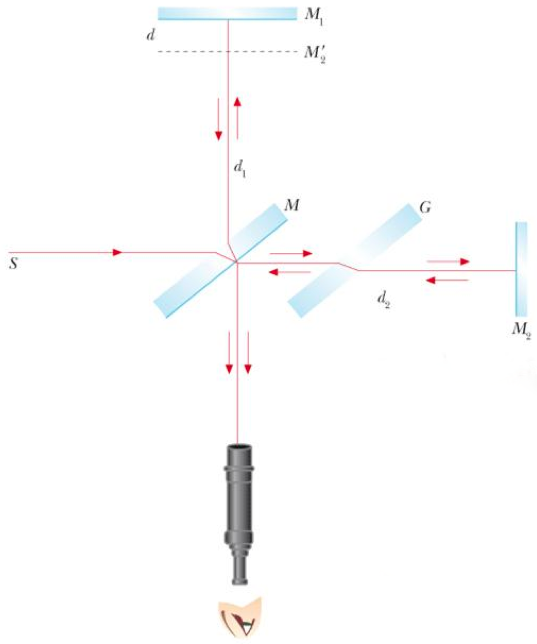
\includegraphics[width=4in]{immagini/michelson.png}
\end{center}
Se non ci fosse $G$ la differenza di fase tra un raggio e l'altro dovuto al diverso spessore di vetro attraversato dipenderebbe la lunghezza d'onda, perché l'indice di rifrazione dipende da $\lambda$. In luce monocromatica $G$ non sarebbe indispensabile.

Se i due specchi sono esattamente perpendicolari tra loro, l'effetto osservato è equivalente a quello di una lamina d'aria di spessore $d=d_1-d_2$: la luce proveniente da $M_2$ gioca il ruolo di luce riflessa sulla superficie inferiore della lamina, quella proveniente da $M_1$ di luce riflessa sulla faccia superiore della lamina.

Si osservano \b{frange di uguale inclinazione circolari con il centro chiaro} perché non ci sono cause aggiuntive di sfasamento. La differenza di cammino è $\Delta r=2d\cos{\theta_i}=2\(d_1-d_2\)\cos{\theta_i}$ e si hanno massimi e minimi di intensità riflessa:
\begin{equation}\begin{split}
\textrm{max}, \qquad 2d\cos{\theta_i}=m\lambda, \qquad \cos{\theta_i}=m\frac{\lambda}{2d}
\end{split}\end{equation}
\begin{equation}\begin{split}
\textrm{min}, \qquad 2d\cos{\theta_i}=\(2m'+1\)\frac{\lambda}{2}, \qquad \cos{\theta_i}=\(2m'+1\)\frac{\lambda}{4d}.
\end{split}\end{equation}